\documentclass{article}
\usepackage{pgfplots}
\pgfplotsset{compat=1.17}

\begin{document}

\begin{figure}[h]
    \centering
    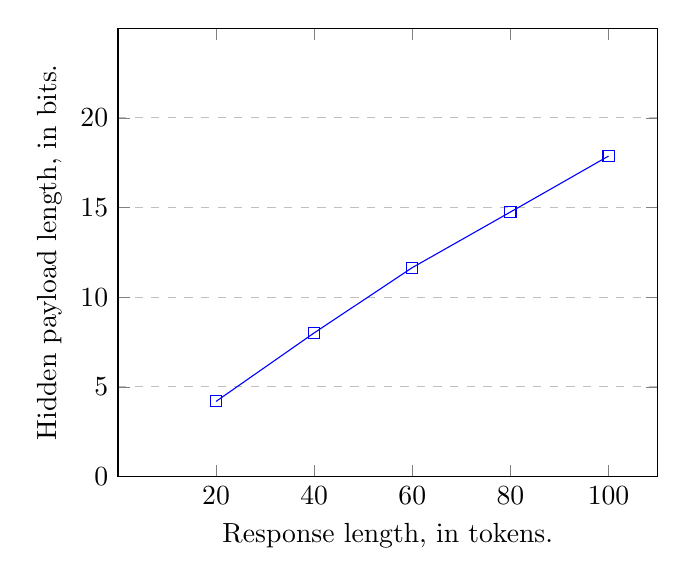
\begin{tikzpicture}
        \begin{axis}[
            xlabel={Response length, in tokens.},
            ylabel={Hidden payload length, in bits.},
            xmin=0, xmax=110,
            ymin=0, ymax=25,
            xtick={20,40,60,80,100},
            ytick={0,5,10,15,20},
            legend pos=north west,
            ymajorgrids=true,
            grid style=dashed,
        ]
        \addplot[
            color=blue,
            mark=square,
            ]
            coordinates {
                (20,4.19)
                (40,8.01)
                (60,11.65)
                (80,14.75)
                (100,17.87)
            };
        \end{axis}
    \end{tikzpicture}
    \caption{Plot of the number of successfully hidden payload bits, by length of response. Experiments ran on GPT-2 with a random choice of an example prompt taken from the OpenAI website. The experiment was performed 100 times for each response length.}
    \label{fig:hidden_payload_length}
\end{figure}

\end{document}